\documentclass[journal,12pt,twocolumn]{IEEEtran}

\usepackage{setspace}
\usepackage{gensymb}

\singlespacing


\usepackage[cmex10]{amsmath}

\usepackage{amsthm}

\usepackage{mathrsfs}
\usepackage{txfonts}
\usepackage{stfloats}
\usepackage{bm}
\usepackage{cite}
\usepackage{cases}
\usepackage{subfig}

\usepackage{longtable}
\usepackage{multirow}

\usepackage{enumitem}
\usepackage{mathtools}
\usepackage{steinmetz}
\usepackage{tikz}
\usepackage{circuitikz}
\usepackage{verbatim}
\usepackage{tfrupee}
\usepackage[breaklinks=true]{hyperref}
\usepackage{graphicx}
\usepackage{tkz-euclide}

\usetikzlibrary{calc,math}
\usepackage{listings}
    \usepackage{color}                                            %%
    \usepackage{array}                                            %%
    \usepackage{longtable}                                        %%
    \usepackage{calc}                                             %%
    \usepackage{multirow}                                         %%
    \usepackage{hhline}                                           %%
    \usepackage{ifthen}                                           %%
    \usepackage{lscape}     
\usepackage{multicol}
\usepackage{chngcntr}

\DeclareMathOperator*{\Res}{Res}

\renewcommand\thesection{\arabic{section}}
\renewcommand\thesubsection{\thesection.\arabic{subsection}}
\renewcommand\thesubsubsection{\thesubsection.\arabic{subsubsection}}

\renewcommand\thesectiondis{\arabic{section}}
\renewcommand\thesubsectiondis{\thesectiondis.\arabic{subsection}}
\renewcommand\thesubsubsectiondis{\thesubsectiondis.\arabic{subsubsection}}


\hyphenation{op-tical net-works semi-conduc-tor}
\def\inputGnumericTable{}                                 %%

\lstset{
%language=C,
frame=single, 
breaklines=true,
columns=fullflexible
}
\begin{document}


\newtheorem{theorem}{Theorem}[section]
\newtheorem{problem}{Problem}
\newtheorem{proposition}{Proposition}[section]
\newtheorem{lemma}{Lemma}[section]
\newtheorem{corollary}[theorem]{Corollary}
\newtheorem{example}{Example}[section]
\newtheorem{definition}[problem]{Definition}

\newcommand{\BEQA}{\begin{eqnarray}}
\newcommand{\EEQA}{\end{eqnarray}}
\newcommand{\define}{\stackrel{\triangle}{=}}
\bibliographystyle{IEEEtran}
\providecommand{\mbf}{\mathbf}
\providecommand{\pr}[1]{\ensuremath{\Pr\left(#1\right)}}
\providecommand{\qfunc}[1]{\ensuremath{Q\left(#1\right)}}
\providecommand{\sbrak}[1]{\ensuremath{{}\left[#1\right]}}
\providecommand{\lsbrak}[1]{\ensuremath{{}\left[#1\right.}}
\providecommand{\rsbrak}[1]{\ensuremath{{}\left.#1\right]}}
\providecommand{\brak}[1]{\ensuremath{\left(#1\right)}}
\providecommand{\lbrak}[1]{\ensuremath{\left(#1\right.}}
\providecommand{\rbrak}[1]{\ensuremath{\left.#1\right)}}
\providecommand{\cbrak}[1]{\ensuremath{\left\{#1\right\}}}
\providecommand{\lcbrak}[1]{\ensuremath{\left\{#1\right.}}
\providecommand{\rcbrak}[1]{\ensuremath{\left.#1\right\}}}
\theoremstyle{remark}
\newtheorem{rem}{Remark}
\newcommand{\sgn}{\mathop{\mathrm{sgn}}}
\providecommand{\abs}[1]{\vert#1\vert}
\providecommand{\res}[1]{\Res\displaylimits_{#1}} 
\providecommand{\norm}[1]{\Vert#1\rVert}
%\providecommand{\norm}[1]{\lVert#1\rVert}
\providecommand{\mtx}[1]{\mathbf{#1}}
\providecommand{\mean}[1]{E[ #1 ]}
\providecommand{\fourier}{\overset{\mathcal{F}}{ \rightleftharpoons}}
%\providecommand{\hilbert}{\overset{\mathcal{H}}{ \rightleftharpoons}}
\providecommand{\system}{\overset{\mathcal{H}}{ \longleftrightarrow}}
	%\newcommand{\solution}[2]{\textbf{Solution:}{#1}}
\newcommand{\solution}{\noindent \textbf{Solution: }}
\newcommand{\cosec}{\,\text{cosec}\,}
\providecommand{\dec}[2]{\ensuremath{\overset{#1}{\underset{#2}{\gtrless}}}}
\newcommand{\myvec}[1]{\ensuremath{\begin{pmatrix}#1\end{pmatrix}}}
\newcommand{\mydet}[1]{\ensuremath{\begin{vmatrix}#1\end{vmatrix}}}
\numberwithin{equation}{subsection}
\makeatletter
\@addtoreset{figure}{problem}
\makeatother
\let\StandardTheFigure\thefigure
\let\vec\mathbf
\renewcommand{\thefigure}{\theproblem}
\def\putbox#1#2#3{\makebox[0in][l]{\makebox[#1][l]{}\raisebox{\baselineskip}[0in][0in]{\raisebox{#2}[0in][0in]{#3}}}}
     \def\rightbox#1{\makebox[0in][r]{#1}}
     \def\centbox#1{\makebox[0in]{#1}}
     \def\topbox#1{\raisebox{-\baselineskip}[0in][0in]{#1}}
     \def\midbox#1{\raisebox{-0.5\baselineskip}[0in][0in]{#1}}
\vspace{3cm}
\title{ASSIGNMENT-2}
\author{K.NIKHITHA}
\maketitle
\newpage
\bigskip
\renewcommand{\thefigure}{\theenumi}
\renewcommand{\thetable}{\theenumi}
Download all python codes from 
\begin{lstlisting}
https://github.com/K.NIKHITHA/Assignment-2/blob/main/ASSIGNMENT2/assignment2.py
\end{lstlisting}
%
and latex-tikz codes from 
%
\begin{lstlisting}
https://github.com/K.NIKHITHA/Assignment-2/blob/main/ASSIGNMENT2/main.tex
\end{lstlisting}
%
\section{Question No. 2.44}
Construct TRUE where $TR = 3.5, RU = 3, UE = 4, \angle R = 75 \degree$ and $\angle U = 120 \degree$.
%
\section{SOLUTION}
\begin{enumerate}
\item Let us assume vertices of given quadrilateral $TRUE$ as $\vec{T}$,$\vec{R}$,$\vec{U}$ and $\vec{E}$.
\item Let us generalize the given data:
    \begin{align}
    &\angle R= 75\degree=\theta \label{eq1}
    \\
    &\angle U= 120\degree=\alpha \label{eq2}
    \\
    &\norm{\vec{T}-\vec{R}} =3.5=a \label{eq3}
    \\
    &\norm{\vec{U}-\vec{R}} =3=b \label{eq4}
    \\
     &\norm{\vec{E}-\vec{U}} =4=c \label{eq5}
    \end{align}
\begin{itemize}
\item For this quadrilateral $TRUE$ we have,
\begin{align}
\angle R +\angle U = 75\degree + 120\degree =195\degree
\end{align}
\item Let, \begin{align}
    &\vec{R}=\myvec{0\\0}, \vec{U}=\myvec{3\\0}
\end{align}
\end{itemize}
\begin{lemma}
\label{lemma}
The coordinates of $\vec{T}$ and  $\vec{E}$ can be written as follows:
\begin{align}
  & \vec{T} = C \vec{u}  \quad \brak{\because \vec{R}=\myvec{0\\0}} \label{eq a}
\\
  & \vec{E} =\vec{U} + a \vec{r} \label{eq b}
\end{align}
 \item Let us define r,u as:
\begin{align}
 \vec{r} = \myvec{\cos R \\\sin R } ,\vec{u} = \myvec{\cos U\\\sin U }
\end{align}
\end{lemma}
\begin{itemize}
\item For finding coordinates of T:-
\end{itemize}
 Putting \eqref{eq1} and \eqref{eq3} in \eqref{eq a} we get,
\begin{align}
&\implies \vec{T}=4\myvec{\cos 120 \\\sin 120 }
\\
&\implies \vec{T}=\myvec{-2\\3.46}
\end{align}
\begin{itemize}
\item For finding coordinates of E:-
\end{itemize}
 Putting \eqref{eq2} and \eqref{eq5} in \eqref{eq b} we get,
\begin{align}
&\implies \vec{E}=\myvec{3\\0} + 3.5\myvec{\cos 75 \\\sin 75 }
\\
&\implies \vec{E}=\myvec{3\\0} + \myvec{0.90\\3.38}
\\
&\implies \vec{E}=\myvec{3.39\\3.38}
\end{align}
\begin{itemize}
\item Now,the vertices of given Quadrilateral TRUE can be written as,
\end{itemize}
\begin{align}
 \vec{T}=\myvec{-2\\3.46},\vec{R} = \myvec{0\\0}, \vec{U}=\myvec{3\\0},\vec{E}=\myvec{3.39\\3.38}
\end{align}
    \item On constructing the quadrilateral $TRUE$ we get:
\numberwithin{figure}{section}
\begin{figure}[!ht]
\centering
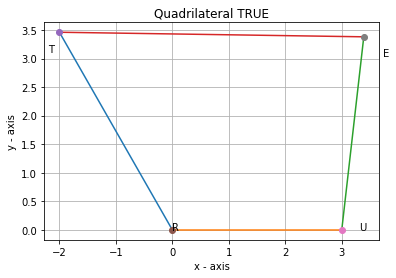
\includegraphics[ width=\columnwidth]{FIG.png}
\caption{Quadrilateral TRUE}
\label{fig:Quadrilateral TRUE}	
\end{figure}
\end{enumerate} 
\end{document}


\end{document}
